% Options for packages loaded elsewhere
\PassOptionsToPackage{unicode}{hyperref}
\PassOptionsToPackage{hyphens}{url}
%
\documentclass[
]{article}
\usepackage{lmodern}
\usepackage{amssymb,amsmath}
\usepackage{ifxetex,ifluatex}
\ifnum 0\ifxetex 1\fi\ifluatex 1\fi=0 % if pdftex
  \usepackage[T1]{fontenc}
  \usepackage[utf8]{inputenc}
  \usepackage{textcomp} % provide euro and other symbols
\else % if luatex or xetex
  \usepackage{unicode-math}
  \defaultfontfeatures{Scale=MatchLowercase}
  \defaultfontfeatures[\rmfamily]{Ligatures=TeX,Scale=1}
\fi
% Use upquote if available, for straight quotes in verbatim environments
\IfFileExists{upquote.sty}{\usepackage{upquote}}{}
\IfFileExists{microtype.sty}{% use microtype if available
  \usepackage[]{microtype}
  \UseMicrotypeSet[protrusion]{basicmath} % disable protrusion for tt fonts
}{}
\makeatletter
\@ifundefined{KOMAClassName}{% if non-KOMA class
  \IfFileExists{parskip.sty}{%
    \usepackage{parskip}
  }{% else
    \setlength{\parindent}{0pt}
    \setlength{\parskip}{6pt plus 2pt minus 1pt}}
}{% if KOMA class
  \KOMAoptions{parskip=half}}
\makeatother
\usepackage{xcolor}
\IfFileExists{xurl.sty}{\usepackage{xurl}}{} % add URL line breaks if available
\IfFileExists{bookmark.sty}{\usepackage{bookmark}}{\usepackage{hyperref}}
\hypersetup{
  pdftitle={Ballistic Trajectory with Drag},
  pdfauthor={Ken Harmon},
  hidelinks,
  pdfcreator={LaTeX via pandoc}}
\urlstyle{same} % disable monospaced font for URLs
\usepackage[margin=1in]{geometry}
\usepackage{color}
\usepackage{fancyvrb}
\newcommand{\VerbBar}{|}
\newcommand{\VERB}{\Verb[commandchars=\\\{\}]}
\DefineVerbatimEnvironment{Highlighting}{Verbatim}{commandchars=\\\{\}}
% Add ',fontsize=\small' for more characters per line
\usepackage{framed}
\definecolor{shadecolor}{RGB}{248,248,248}
\newenvironment{Shaded}{\begin{snugshade}}{\end{snugshade}}
\newcommand{\AlertTok}[1]{\textcolor[rgb]{0.94,0.16,0.16}{#1}}
\newcommand{\AnnotationTok}[1]{\textcolor[rgb]{0.56,0.35,0.01}{\textbf{\textit{#1}}}}
\newcommand{\AttributeTok}[1]{\textcolor[rgb]{0.77,0.63,0.00}{#1}}
\newcommand{\BaseNTok}[1]{\textcolor[rgb]{0.00,0.00,0.81}{#1}}
\newcommand{\BuiltInTok}[1]{#1}
\newcommand{\CharTok}[1]{\textcolor[rgb]{0.31,0.60,0.02}{#1}}
\newcommand{\CommentTok}[1]{\textcolor[rgb]{0.56,0.35,0.01}{\textit{#1}}}
\newcommand{\CommentVarTok}[1]{\textcolor[rgb]{0.56,0.35,0.01}{\textbf{\textit{#1}}}}
\newcommand{\ConstantTok}[1]{\textcolor[rgb]{0.00,0.00,0.00}{#1}}
\newcommand{\ControlFlowTok}[1]{\textcolor[rgb]{0.13,0.29,0.53}{\textbf{#1}}}
\newcommand{\DataTypeTok}[1]{\textcolor[rgb]{0.13,0.29,0.53}{#1}}
\newcommand{\DecValTok}[1]{\textcolor[rgb]{0.00,0.00,0.81}{#1}}
\newcommand{\DocumentationTok}[1]{\textcolor[rgb]{0.56,0.35,0.01}{\textbf{\textit{#1}}}}
\newcommand{\ErrorTok}[1]{\textcolor[rgb]{0.64,0.00,0.00}{\textbf{#1}}}
\newcommand{\ExtensionTok}[1]{#1}
\newcommand{\FloatTok}[1]{\textcolor[rgb]{0.00,0.00,0.81}{#1}}
\newcommand{\FunctionTok}[1]{\textcolor[rgb]{0.00,0.00,0.00}{#1}}
\newcommand{\ImportTok}[1]{#1}
\newcommand{\InformationTok}[1]{\textcolor[rgb]{0.56,0.35,0.01}{\textbf{\textit{#1}}}}
\newcommand{\KeywordTok}[1]{\textcolor[rgb]{0.13,0.29,0.53}{\textbf{#1}}}
\newcommand{\NormalTok}[1]{#1}
\newcommand{\OperatorTok}[1]{\textcolor[rgb]{0.81,0.36,0.00}{\textbf{#1}}}
\newcommand{\OtherTok}[1]{\textcolor[rgb]{0.56,0.35,0.01}{#1}}
\newcommand{\PreprocessorTok}[1]{\textcolor[rgb]{0.56,0.35,0.01}{\textit{#1}}}
\newcommand{\RegionMarkerTok}[1]{#1}
\newcommand{\SpecialCharTok}[1]{\textcolor[rgb]{0.00,0.00,0.00}{#1}}
\newcommand{\SpecialStringTok}[1]{\textcolor[rgb]{0.31,0.60,0.02}{#1}}
\newcommand{\StringTok}[1]{\textcolor[rgb]{0.31,0.60,0.02}{#1}}
\newcommand{\VariableTok}[1]{\textcolor[rgb]{0.00,0.00,0.00}{#1}}
\newcommand{\VerbatimStringTok}[1]{\textcolor[rgb]{0.31,0.60,0.02}{#1}}
\newcommand{\WarningTok}[1]{\textcolor[rgb]{0.56,0.35,0.01}{\textbf{\textit{#1}}}}
\usepackage{longtable,booktabs}
% Correct order of tables after \paragraph or \subparagraph
\usepackage{etoolbox}
\makeatletter
\patchcmd\longtable{\par}{\if@noskipsec\mbox{}\fi\par}{}{}
\makeatother
% Allow footnotes in longtable head/foot
\IfFileExists{footnotehyper.sty}{\usepackage{footnotehyper}}{\usepackage{footnote}}
\makesavenoteenv{longtable}
\usepackage{graphicx,grffile}
\makeatletter
\def\maxwidth{\ifdim\Gin@nat@width>\linewidth\linewidth\else\Gin@nat@width\fi}
\def\maxheight{\ifdim\Gin@nat@height>\textheight\textheight\else\Gin@nat@height\fi}
\makeatother
% Scale images if necessary, so that they will not overflow the page
% margins by default, and it is still possible to overwrite the defaults
% using explicit options in \includegraphics[width, height, ...]{}
\setkeys{Gin}{width=\maxwidth,height=\maxheight,keepaspectratio}
% Set default figure placement to htbp
\makeatletter
\def\fps@figure{htbp}
\makeatother
\setlength{\emergencystretch}{3em} % prevent overfull lines
\providecommand{\tightlist}{%
  \setlength{\itemsep}{0pt}\setlength{\parskip}{0pt}}
\setcounter{secnumdepth}{-\maxdimen} % remove section numbering

\title{Ballistic Trajectory with Drag}
\author{Ken Harmon}
\date{2020 May 31}

\begin{document}
\maketitle

\hypertarget{section}{%
\section{}\label{section}}

Ballistic Trajectory with Drag

\emph{No Drag}

Firing Artillery is an interesting proposition. Hitting the target with
as few rounds as possible is very important. Each round fired comes at a
cost. Besides the monetary cost, each round draws unwanted attention
from the enemy. Therefore, each round needs to be carefully considered.
Each target needs to provide enough payoff to outweigh the cost and the
calculations for each round needs to be meticulous and timely in order
to have as little adjustment as possible and requiring subsequent
rounds.

The initial physics behind firing artillery seems pretty straight
forward. Initial velocity at some angle: the initial velocity vector V

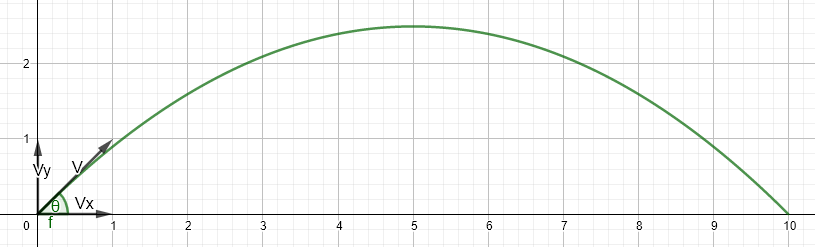
\includegraphics{media/bdc6aece00f34d9fb2f177df1c70e766.png}

We analyze the components of that initial vector separately Vx and Vy.

\[V_{x} = Vcos\theta\] \[V_{y} = Vsin\theta\]

If there were no drag on the round, Vx would remain constant and Vy
would be affected only by gravity. For this paper,
\[x_{0} = y_{0} = t_{0} = x_{f} =
y_{f} = 0\]

\[\frac{\text{dx}}{\text{dt}} = \ Vcos\theta,\ \ x = Vtcos\theta,\ \
\frac{\text{dy}}{\text{dt}} = \ Vsin\theta - gt,\ \ y = Vtsin\theta -
\frac{1}{2}gt^{2}\]

So, for a given initial velocity, in order to hit the target, we need x
to equal the range (r) to the target at the same time y equals the
height of the target (zero in this case).

\[\frac{r}{\text{Vcosθ}} = t = \frac{2Vsin\theta}{g} \rightarrow r =
\frac{2V^{2}\text{sinθcosθ}}{g} = \frac{V^{2}sin2\theta}{g}\]

So, for a target at a given range and a round fired at a set velocity,
we know the angle that must be shot. \[\theta = \frac{1}{2}arcsin\left(
\frac{\text{rg}}{V^{2}} \right)\]

We also know the maximum height (H) of the round happens at half the
range and half the time.

\[If\ halftime = \frac{\text{Vsinθ}}{g}\] , then
\[H =\frac{V^{2}\sin^{2}\theta}{2g}\]

For example, to hit a target at 15km with an initial velocity of 671
m/s, the initial angle needs to be .1664 radians, 9.54 degrees, or 169.7
mils. Time of flight is 22.668. Max height is 629.87 m at 11.3339
seconds. Impact angle is -169.7 mils. Impact velocity is 671 m/s.

This is all very predictable, but there is a great deal of drag so
things change.

\emph{Drag}

If there is drag on the round, there are many variables that affect the
velocity of the round. Velocity in the x direction is no longer
constant. I get these formulas from Peter Chudinov from the journal of
Physics\footnote{\url{https://iopscience.iop.org/article/10.1088/1742-6596/1287/1/012032}}.

The drag constant
\[k = \frac{\rho_{a}c_{d}S}{2mg} = \frac{1}{V_{t}^{2}}\];

ρ\emph{a} is the air density, \emph{cd} is the drag factor for a sphere,
\emph{S} is the cross-section area of the object, and \emph{Vt} is the
terminal velocity.

I will treat k as a constant even though ρ changes with altitude which
may be significant with artillery shots; in this case k could become a
function. All variables are functions of θ. Theta is the angle of
trajectory that varies throughout the flight.

Launch angle: \[\text{θϵ}\left\lbrack 0,\frac{\pi}{2} \right\rbrack\]
Impact angle: \[- \text{θϵ}\left\lbrack 0,\frac{\pi}{2} \right\rbrack\]

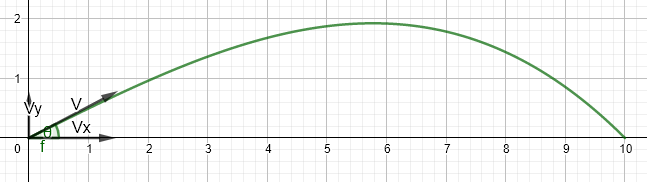
\includegraphics{media/09aa336ef56776834ee2eced9ecb01ff.png}

Here are the functions I am going to use to predict artillery shots
given and initial velocity and launch angle.

These first two equations I can compute directly from θ.

\begin{enumerate}
\def\labelenumi{\arabic{enumi}.}
\item
  \[f\left( \theta \right) = \frac{\text{sinθ}}{\cos^{2}\theta} + ln\left(
  \tan\left( \frac{\theta}{2} + \frac{\pi}{4} \right) \right)\]
\item
  \[V\left( \theta \right) = \frac{V_{0}\cos\theta_{0}}{\text{cosθ}\sqrt{1 +
  kV_{0}^{2}\cos^{2}\theta_{0}\left( f\left( \theta_{0} \right) - f\left(
  \theta \right) \right)}}\]
\end{enumerate}

The following formulas I cannot compute directly but I can get a
numerical solution for each θ.

The velocity in the x and y directions is now based off of instantaneous
velocity and trajectory angle; not just initial velocity and launch
angle.

\begin{enumerate}
\def\labelenumi{\arabic{enumi}.}
\tightlist
\item
  \[\frac{\text{dx}}{\text{dt}} = Vcos\theta,
  \frac{\text{dy}}{\text{dt}} = Vsin\theta,
  \frac{\text{dθ}}{\text{dt}} = \frac{- gcos\theta}{V},
  \frac{\text{dV}}{\text{dt}} = - gsin\theta - gkV^{2}\]
\end{enumerate}

Now convert all these so they are in terms of θ:

\begin{enumerate}
\def\labelenumi{\arabic{enumi}.}
\item
  \[\frac{\text{dV}}{\text{dθ}} = Vtan\theta + \frac{kV^{3}}{\text{cosθ}},\ \
  \ \ \frac{\text{dx}}{\text{dθ}} = \frac{V^{2}}{- g},\ \ \ \
  \frac{\text{dy}}{\text{dθ}} = \frac{V^{2}}{- g}tan\theta,\ \ \ \
  \frac{\text{dt}}{\text{dθ}} = \frac{V}{- gcos\theta}\]
\item
  \[x = \int_{\theta_{0}}^{\theta}{\frac{V^{2}}{- g}\text{dθ}},\ \ \ \ y =
  \int_{\theta_{0}}^{\theta}{\frac{V^{2}}{- g}\text{tanθ dθ}},\ \ \ \ t =
  \int_{\theta_{0}}^{\theta}{\frac{V}{- gcos\theta}\text{dθ}}\]
\end{enumerate}

Once I have and instantaneous altitude, I can alter k for appropriate
air pressure.

\emph{Attempt at prediction}

Actual shot data that I am trying to match: Initial velocity 547 m/s at
an initial angle of (330.2 mils). My prediction needs to hit a level
target at 10000 m in 28.8 seconds while reaching a maximum altitude of
1070 m. Also, impact angle of (-483 mils) with and impact velocity of
298 m/s.

\begin{Shaded}
\begin{Highlighting}[]
\NormalTok{v0 <-}\StringTok{ }\DecValTok{547} \CommentTok{# initial velocity in m/s for M795 with M232A1 4H}
\NormalTok{am0 <-}\StringTok{ }\FloatTok{330.2} \CommentTok{# QE in mils for a level 15000 m shot}

\NormalTok{th0 <-}\StringTok{ }\NormalTok{am0 }\OperatorTok{*}\StringTok{ }\NormalTok{pi }\OperatorTok{/}\StringTok{ }\DecValTok{3200} \CommentTok{# initial angle in radians}
\NormalTok{x0 <-}\StringTok{ }\DecValTok{0} \CommentTok{#Initial x}
\NormalTok{y0 <-}\StringTok{ }\DecValTok{0} \CommentTok{# initial y}
\NormalTok{t0 <-}\StringTok{ }\DecValTok{0} \CommentTok{# initial time}
\NormalTok{g <-}\StringTok{ }\FloatTok{9.80665} \CommentTok{# gravitational force in m/s/s}
\NormalTok{press <-}\StringTok{ }\KeywordTok{data.frame}\NormalTok{(}\KeywordTok{cbind}\NormalTok{(}
  \DataTypeTok{alt =} \KeywordTok{c}\NormalTok{(}\DecValTok{0}\NormalTok{,}\DecValTok{200}\NormalTok{,}\DecValTok{500}\NormalTok{,}\DecValTok{1000}\NormalTok{,}\DecValTok{1500}\NormalTok{,}\DecValTok{2000}\NormalTok{,}\DecValTok{2500}\NormalTok{,}\DecValTok{3000}\NormalTok{,}\DecValTok{3500}\NormalTok{,}
          \DecValTok{4000}\NormalTok{,}\DecValTok{4500}\NormalTok{,}\DecValTok{5000}\NormalTok{,}\DecValTok{6000}\NormalTok{,}\DecValTok{7000}\NormalTok{,}\DecValTok{8000}\NormalTok{,}\DecValTok{9000}\NormalTok{),}
  \DataTypeTok{rho =} \KeywordTok{c}\NormalTok{(}\FloatTok{1.2250}\NormalTok{,}\FloatTok{1.2133}\NormalTok{,}\FloatTok{1.1844}\NormalTok{,}\FloatTok{1.1392}\NormalTok{,}\FloatTok{1.0846}\NormalTok{,}\FloatTok{1.0320}\NormalTok{,}
          \FloatTok{.9569}\NormalTok{,.}\DecValTok{8632}\NormalTok{,.}\DecValTok{7768}\NormalTok{,.}\DecValTok{6971}\NormalTok{,.}\DecValTok{5895}\NormalTok{,.}\DecValTok{4664}\NormalTok{,.}\DecValTok{3612}\NormalTok{,.}\DecValTok{2655}\NormalTok{,.}\DecValTok{1937}\NormalTok{,.}\DecValTok{1413}\NormalTok{)))}
\NormalTok{c.press <-}\StringTok{ }\KeywordTok{glm}\NormalTok{(rho}\OperatorTok{~}\KeywordTok{poly}\NormalTok{(alt,}\DecValTok{6}\NormalTok{,}\DataTypeTok{raw=}\OtherTok{TRUE}\NormalTok{), }\DataTypeTok{data =}\NormalTok{ press)}
\NormalTok{pk <-}\StringTok{ }\FloatTok{.000006} \OperatorTok{*}\StringTok{ }\FloatTok{46.94681}
\NormalTok{m <-}\StringTok{ }\FloatTok{46.94681} \CommentTok{#mass in kg}
\NormalTok{rho <-}\StringTok{ }\KeywordTok{as.numeric}\NormalTok{(}\KeywordTok{predict}\NormalTok{(c.press, }\KeywordTok{data.frame}\NormalTok{(}\DataTypeTok{alt =}\NormalTok{ y0), }\DataTypeTok{type =} \StringTok{"response"}\NormalTok{))}
\NormalTok{k <-}\StringTok{ }\NormalTok{rho}\OperatorTok{*}\NormalTok{pk}\OperatorTok{/}\NormalTok{m }\CommentTok{# is the drag constant at 0 alt}
\CommentTok{#k <- .0000075 # Drag}


\NormalTok{traj <-}\StringTok{ }\KeywordTok{data.frame}\NormalTok{(}\KeywordTok{matrix}\NormalTok{(}\DataTypeTok{ncol =} \DecValTok{7}\NormalTok{))}
\KeywordTok{colnames}\NormalTok{(traj)=}\KeywordTok{c}\NormalTok{(}\StringTok{"Time s"}\NormalTok{,}\StringTok{"k"}\NormalTok{,}\StringTok{"Vel m/s"}\NormalTok{,}\StringTok{"Angle r"}\NormalTok{,}\StringTok{"Angle mils"}\NormalTok{,}\StringTok{"Range m"}\NormalTok{,}\StringTok{"Alt m"}\NormalTok{)}
\NormalTok{t <-}\StringTok{ }\NormalTok{t0}
\NormalTok{v <-}\StringTok{ }\NormalTok{v0}
\NormalTok{th <-}\StringTok{ }\NormalTok{th0}
\NormalTok{x <-}\StringTok{ }\NormalTok{x0}
\NormalTok{y <-}\StringTok{ }\NormalTok{y0}
\NormalTok{firstrow <-}\StringTok{ }\KeywordTok{c}\NormalTok{(t,k,v,th,th}\OperatorTok{*}\DecValTok{3200}\OperatorTok{/}\NormalTok{pi,x,y)}
\NormalTok{traj[}\DecValTok{1}\NormalTok{,] <-}\StringTok{ }\NormalTok{firstrow}
\NormalTok{dt <-}\StringTok{ }\FloatTok{.1}
\ControlFlowTok{while}\NormalTok{ (y }\OperatorTok{>}\StringTok{ }\DecValTok{-1}\NormalTok{)\{}
\NormalTok{t <-}\StringTok{ }\NormalTok{t }\OperatorTok{+}\StringTok{ }\NormalTok{dt}
\NormalTok{rho <-}\StringTok{ }\KeywordTok{as.numeric}\NormalTok{(}\KeywordTok{predict}\NormalTok{(c.press, }\KeywordTok{data.frame}\NormalTok{(}\DataTypeTok{alt =}\NormalTok{ y), }\DataTypeTok{type =} \StringTok{"response"}\NormalTok{))}
\NormalTok{k <-}\StringTok{ }\NormalTok{rho}\OperatorTok{*}\NormalTok{pk}\OperatorTok{/}\NormalTok{m }\CommentTok{# is the drag constant at y alt}
\NormalTok{v <-}\StringTok{ }\NormalTok{v }\OperatorTok{-}\StringTok{ }\NormalTok{(}\KeywordTok{sin}\NormalTok{(th) }\OperatorTok{+}\StringTok{ }\NormalTok{k}\OperatorTok{*}\NormalTok{v}\OperatorTok{^}\DecValTok{2}\NormalTok{) }\OperatorTok{*}\StringTok{ }\NormalTok{g }\OperatorTok{*}\StringTok{ }\NormalTok{dt}
\NormalTok{th <-}\StringTok{ }\NormalTok{th }\OperatorTok{-}\StringTok{ }\NormalTok{(g}\OperatorTok{*}\KeywordTok{cos}\NormalTok{(th)}\OperatorTok{/}\NormalTok{v)}\OperatorTok{*}\NormalTok{dt}
\NormalTok{x <-}\StringTok{ }\NormalTok{x }\OperatorTok{+}\StringTok{ }\NormalTok{v}\OperatorTok{*}\NormalTok{dt}\OperatorTok{*}\KeywordTok{cos}\NormalTok{(th)}
\NormalTok{y <-}\StringTok{ }\NormalTok{y }\OperatorTok{+}\StringTok{ }\NormalTok{v}\OperatorTok{*}\NormalTok{dt}\OperatorTok{*}\KeywordTok{sin}\NormalTok{(th)}
\NormalTok{nextrow <-}\StringTok{ }\KeywordTok{c}\NormalTok{(t,k,v,th,th}\OperatorTok{*}\DecValTok{3200}\OperatorTok{/}\NormalTok{pi,x,y)}
\NormalTok{traj <-}\StringTok{ }\KeywordTok{rbind}\NormalTok{(traj,nextrow)}
\NormalTok{\}}
\NormalTok{trajw <-}\StringTok{ }\NormalTok{traj[}\KeywordTok{seq}\NormalTok{(}\DecValTok{1}\NormalTok{, }\KeywordTok{nrow}\NormalTok{(traj), }\DecValTok{10}\NormalTok{), ]}
\NormalTok{traj }\OperatorTok\StringTok{ }\KeywordTok{ggplot}\NormalTok{(}\KeywordTok{aes}\NormalTok{(}\StringTok{`}\DataTypeTok{Range m}\StringTok{`}\NormalTok{,}\StringTok{`}\DataTypeTok{Alt m}\StringTok{`}\NormalTok{))}\OperatorTok{+}\KeywordTok{geom_point}\NormalTok{(}\DataTypeTok{size=}\NormalTok{.}\DecValTok{1}\NormalTok{) }\OperatorTok{+}
\StringTok{  }\KeywordTok{geom_point}\NormalTok{(}\DataTypeTok{data=}\NormalTok{trajw,}\KeywordTok{aes}\NormalTok{(}\StringTok{`}\DataTypeTok{Range m}\StringTok{`}\NormalTok{,}\StringTok{`}\DataTypeTok{Alt m}\StringTok{`}\NormalTok{),}\DataTypeTok{color=}\StringTok{"blue"}\NormalTok{) }\OperatorTok{+}
\StringTok{    }\KeywordTok{coord_fixed}\NormalTok{(}\DataTypeTok{ratio =} \DecValTok{1}\NormalTok{)}
\end{Highlighting}
\end{Shaded}

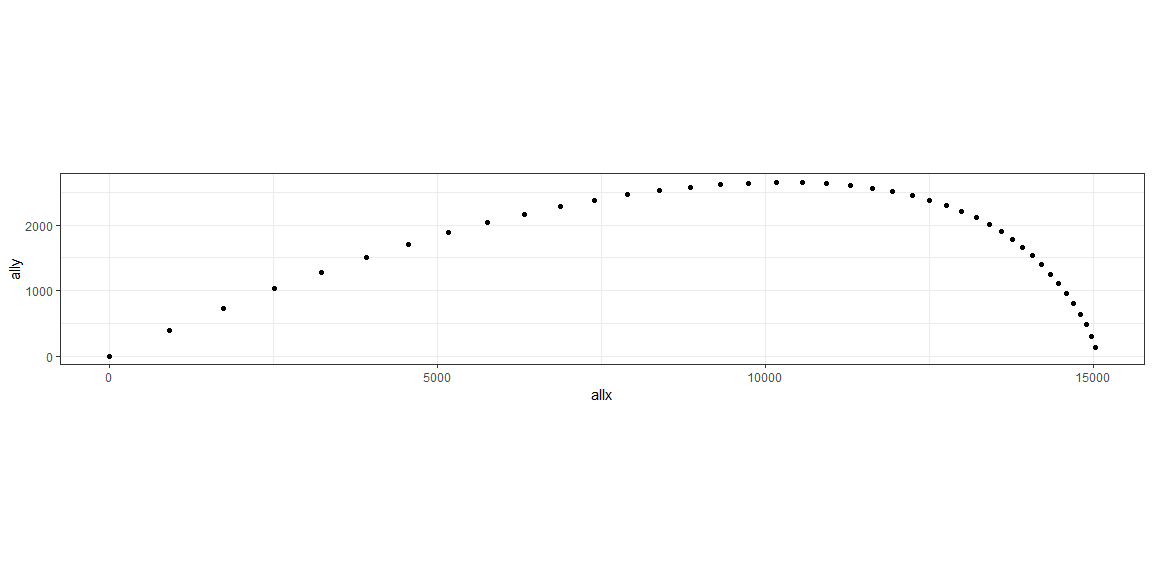
\includegraphics{Trajectory_t_files/figure-latex/try-1.pdf}

\begin{Shaded}
\begin{Highlighting}[]
\KeywordTok{pander}\NormalTok{(trajw)}
\end{Highlighting}
\end{Shaded}

\begin{longtable}[]{@{}cccccccc@{}}
\toprule
\begin{minipage}[b]{0.09\columnwidth}\centering
~\strut
\end{minipage} & \begin{minipage}[b]{0.08\columnwidth}\centering
Time s\strut
\end{minipage} & \begin{minipage}[b]{0.11\columnwidth}\centering
k\strut
\end{minipage} & \begin{minipage}[b]{0.09\columnwidth}\centering
Vel m/s\strut
\end{minipage} & \begin{minipage}[b]{0.10\columnwidth}\centering
Angle r\strut
\end{minipage} & \begin{minipage}[b]{0.12\columnwidth}\centering
Angle mils\strut
\end{minipage} & \begin{minipage}[b]{0.09\columnwidth}\centering
Range m\strut
\end{minipage} & \begin{minipage}[b]{0.09\columnwidth}\centering
Alt m\strut
\end{minipage}\tabularnewline
\midrule
\endhead
\begin{minipage}[t]{0.09\columnwidth}\centering
\textbf{1}\strut
\end{minipage} & \begin{minipage}[t]{0.08\columnwidth}\centering
0\strut
\end{minipage} & \begin{minipage}[t]{0.11\columnwidth}\centering
7.383e-06\strut
\end{minipage} & \begin{minipage}[t]{0.09\columnwidth}\centering
547\strut
\end{minipage} & \begin{minipage}[t]{0.10\columnwidth}\centering
0.3242\strut
\end{minipage} & \begin{minipage}[t]{0.12\columnwidth}\centering
330.2\strut
\end{minipage} & \begin{minipage}[t]{0.09\columnwidth}\centering
0\strut
\end{minipage} & \begin{minipage}[t]{0.09\columnwidth}\centering
0\strut
\end{minipage}\tabularnewline
\begin{minipage}[t]{0.09\columnwidth}\centering
\textbf{11}\strut
\end{minipage} & \begin{minipage}[t]{0.08\columnwidth}\centering
1\strut
\end{minipage} & \begin{minipage}[t]{0.11\columnwidth}\centering
7.281e-06\strut
\end{minipage} & \begin{minipage}[t]{0.09\columnwidth}\centering
523.3\strut
\end{minipage} & \begin{minipage}[t]{0.10\columnwidth}\centering
0.3067\strut
\end{minipage} & \begin{minipage}[t]{0.12\columnwidth}\centering
312.4\strut
\end{minipage} & \begin{minipage}[t]{0.09\columnwidth}\centering
507.5\strut
\end{minipage} & \begin{minipage}[t]{0.09\columnwidth}\centering
165.2\strut
\end{minipage}\tabularnewline
\begin{minipage}[t]{0.09\columnwidth}\centering
\textbf{21}\strut
\end{minipage} & \begin{minipage}[t]{0.08\columnwidth}\centering
2\strut
\end{minipage} & \begin{minipage}[t]{0.11\columnwidth}\centering
7.191e-06\strut
\end{minipage} & \begin{minipage}[t]{0.09\columnwidth}\centering
501.7\strut
\end{minipage} & \begin{minipage}[t]{0.10\columnwidth}\centering
0.2884\strut
\end{minipage} & \begin{minipage}[t]{0.12\columnwidth}\centering
293.7\strut
\end{minipage} & \begin{minipage}[t]{0.09\columnwidth}\centering
996.4\strut
\end{minipage} & \begin{minipage}[t]{0.09\columnwidth}\centering
314.7\strut
\end{minipage}\tabularnewline
\begin{minipage}[t]{0.09\columnwidth}\centering
\textbf{31}\strut
\end{minipage} & \begin{minipage}[t]{0.08\columnwidth}\centering
3\strut
\end{minipage} & \begin{minipage}[t]{0.11\columnwidth}\centering
7.117e-06\strut
\end{minipage} & \begin{minipage}[t]{0.09\columnwidth}\centering
482\strut
\end{minipage} & \begin{minipage}[t]{0.10\columnwidth}\centering
0.2692\strut
\end{minipage} & \begin{minipage}[t]{0.12\columnwidth}\centering
274.2\strut
\end{minipage} & \begin{minipage}[t]{0.09\columnwidth}\centering
1468\strut
\end{minipage} & \begin{minipage}[t]{0.09\columnwidth}\centering
449.4\strut
\end{minipage}\tabularnewline
\begin{minipage}[t]{0.09\columnwidth}\centering
\textbf{41}\strut
\end{minipage} & \begin{minipage}[t]{0.08\columnwidth}\centering
4\strut
\end{minipage} & \begin{minipage}[t]{0.11\columnwidth}\centering
7.054e-06\strut
\end{minipage} & \begin{minipage}[t]{0.09\columnwidth}\centering
463.9\strut
\end{minipage} & \begin{minipage}[t]{0.10\columnwidth}\centering
0.2491\strut
\end{minipage} & \begin{minipage}[t]{0.12\columnwidth}\centering
253.7\strut
\end{minipage} & \begin{minipage}[t]{0.09\columnwidth}\centering
1925\strut
\end{minipage} & \begin{minipage}[t]{0.09\columnwidth}\centering
569.9\strut
\end{minipage}\tabularnewline
\begin{minipage}[t]{0.09\columnwidth}\centering
\textbf{51}\strut
\end{minipage} & \begin{minipage}[t]{0.08\columnwidth}\centering
5\strut
\end{minipage} & \begin{minipage}[t]{0.11\columnwidth}\centering
6.999e-06\strut
\end{minipage} & \begin{minipage}[t]{0.09\columnwidth}\centering
447.2\strut
\end{minipage} & \begin{minipage}[t]{0.10\columnwidth}\centering
0.2281\strut
\end{minipage} & \begin{minipage}[t]{0.12\columnwidth}\centering
232.4\strut
\end{minipage} & \begin{minipage}[t]{0.09\columnwidth}\centering
2366\strut
\end{minipage} & \begin{minipage}[t]{0.09\columnwidth}\centering
676.9\strut
\end{minipage}\tabularnewline
\begin{minipage}[t]{0.09\columnwidth}\centering
\textbf{61}\strut
\end{minipage} & \begin{minipage}[t]{0.08\columnwidth}\centering
6\strut
\end{minipage} & \begin{minipage}[t]{0.11\columnwidth}\centering
6.952e-06\strut
\end{minipage} & \begin{minipage}[t]{0.09\columnwidth}\centering
431.8\strut
\end{minipage} & \begin{minipage}[t]{0.10\columnwidth}\centering
0.2063\strut
\end{minipage} & \begin{minipage}[t]{0.12\columnwidth}\centering
210.1\strut
\end{minipage} & \begin{minipage}[t]{0.09\columnwidth}\centering
2795\strut
\end{minipage} & \begin{minipage}[t]{0.09\columnwidth}\centering
771\strut
\end{minipage}\tabularnewline
\begin{minipage}[t]{0.09\columnwidth}\centering
\textbf{71}\strut
\end{minipage} & \begin{minipage}[t]{0.08\columnwidth}\centering
7\strut
\end{minipage} & \begin{minipage}[t]{0.11\columnwidth}\centering
6.911e-06\strut
\end{minipage} & \begin{minipage}[t]{0.09\columnwidth}\centering
417.6\strut
\end{minipage} & \begin{minipage}[t]{0.10\columnwidth}\centering
0.1836\strut
\end{minipage} & \begin{minipage}[t]{0.12\columnwidth}\centering
187\strut
\end{minipage} & \begin{minipage}[t]{0.09\columnwidth}\centering
3211\strut
\end{minipage} & \begin{minipage}[t]{0.09\columnwidth}\centering
852.7\strut
\end{minipage}\tabularnewline
\begin{minipage}[t]{0.09\columnwidth}\centering
\textbf{81}\strut
\end{minipage} & \begin{minipage}[t]{0.08\columnwidth}\centering
8\strut
\end{minipage} & \begin{minipage}[t]{0.11\columnwidth}\centering
6.875e-06\strut
\end{minipage} & \begin{minipage}[t]{0.09\columnwidth}\centering
404.5\strut
\end{minipage} & \begin{minipage}[t]{0.10\columnwidth}\centering
0.1601\strut
\end{minipage} & \begin{minipage}[t]{0.12\columnwidth}\centering
163\strut
\end{minipage} & \begin{minipage}[t]{0.09\columnwidth}\centering
3615\strut
\end{minipage} & \begin{minipage}[t]{0.09\columnwidth}\centering
922.4\strut
\end{minipage}\tabularnewline
\begin{minipage}[t]{0.09\columnwidth}\centering
\textbf{91}\strut
\end{minipage} & \begin{minipage}[t]{0.08\columnwidth}\centering
9\strut
\end{minipage} & \begin{minipage}[t]{0.11\columnwidth}\centering
6.845e-06\strut
\end{minipage} & \begin{minipage}[t]{0.09\columnwidth}\centering
392.3\strut
\end{minipage} & \begin{minipage}[t]{0.10\columnwidth}\centering
0.1357\strut
\end{minipage} & \begin{minipage}[t]{0.12\columnwidth}\centering
138.2\strut
\end{minipage} & \begin{minipage}[t]{0.09\columnwidth}\centering
4008\strut
\end{minipage} & \begin{minipage}[t]{0.09\columnwidth}\centering
980.6\strut
\end{minipage}\tabularnewline
\begin{minipage}[t]{0.09\columnwidth}\centering
\textbf{101}\strut
\end{minipage} & \begin{minipage}[t]{0.08\columnwidth}\centering
10\strut
\end{minipage} & \begin{minipage}[t]{0.11\columnwidth}\centering
6.82e-06\strut
\end{minipage} & \begin{minipage}[t]{0.09\columnwidth}\centering
381.1\strut
\end{minipage} & \begin{minipage}[t]{0.10\columnwidth}\centering
0.1105\strut
\end{minipage} & \begin{minipage}[t]{0.12\columnwidth}\centering
112.5\strut
\end{minipage} & \begin{minipage}[t]{0.09\columnwidth}\centering
4392\strut
\end{minipage} & \begin{minipage}[t]{0.09\columnwidth}\centering
1028\strut
\end{minipage}\tabularnewline
\begin{minipage}[t]{0.09\columnwidth}\centering
\textbf{111}\strut
\end{minipage} & \begin{minipage}[t]{0.08\columnwidth}\centering
11\strut
\end{minipage} & \begin{minipage}[t]{0.11\columnwidth}\centering
6.8e-06\strut
\end{minipage} & \begin{minipage}[t]{0.09\columnwidth}\centering
370.6\strut
\end{minipage} & \begin{minipage}[t]{0.10\columnwidth}\centering
0.08446\strut
\end{minipage} & \begin{minipage}[t]{0.12\columnwidth}\centering
86.03\strut
\end{minipage} & \begin{minipage}[t]{0.09\columnwidth}\centering
4765\strut
\end{minipage} & \begin{minipage}[t]{0.09\columnwidth}\centering
1064\strut
\end{minipage}\tabularnewline
\begin{minipage}[t]{0.09\columnwidth}\centering
\textbf{121}\strut
\end{minipage} & \begin{minipage}[t]{0.08\columnwidth}\centering
12\strut
\end{minipage} & \begin{minipage}[t]{0.11\columnwidth}\centering
6.786e-06\strut
\end{minipage} & \begin{minipage}[t]{0.09\columnwidth}\centering
361\strut
\end{minipage} & \begin{minipage}[t]{0.10\columnwidth}\centering
0.05768\strut
\end{minipage} & \begin{minipage}[t]{0.12\columnwidth}\centering
58.75\strut
\end{minipage} & \begin{minipage}[t]{0.09\columnwidth}\centering
5130\strut
\end{minipage} & \begin{minipage}[t]{0.09\columnwidth}\centering
1089\strut
\end{minipage}\tabularnewline
\begin{minipage}[t]{0.09\columnwidth}\centering
\textbf{131}\strut
\end{minipage} & \begin{minipage}[t]{0.08\columnwidth}\centering
13\strut
\end{minipage} & \begin{minipage}[t]{0.11\columnwidth}\centering
6.778e-06\strut
\end{minipage} & \begin{minipage}[t]{0.09\columnwidth}\centering
352.1\strut
\end{minipage} & \begin{minipage}[t]{0.10\columnwidth}\centering
0.03016\strut
\end{minipage} & \begin{minipage}[t]{0.12\columnwidth}\centering
30.72\strut
\end{minipage} & \begin{minipage}[t]{0.09\columnwidth}\centering
5485\strut
\end{minipage} & \begin{minipage}[t]{0.09\columnwidth}\centering
1104\strut
\end{minipage}\tabularnewline
\begin{minipage}[t]{0.09\columnwidth}\centering
\textbf{141}\strut
\end{minipage} & \begin{minipage}[t]{0.08\columnwidth}\centering
14\strut
\end{minipage} & \begin{minipage}[t]{0.11\columnwidth}\centering
6.774e-06\strut
\end{minipage} & \begin{minipage}[t]{0.09\columnwidth}\centering
343.8\strut
\end{minipage} & \begin{minipage}[t]{0.10\columnwidth}\centering
0.001943\strut
\end{minipage} & \begin{minipage}[t]{0.12\columnwidth}\centering
1.979\strut
\end{minipage} & \begin{minipage}[t]{0.09\columnwidth}\centering
5833\strut
\end{minipage} & \begin{minipage}[t]{0.09\columnwidth}\centering
1109\strut
\end{minipage}\tabularnewline
\begin{minipage}[t]{0.09\columnwidth}\centering
\textbf{151}\strut
\end{minipage} & \begin{minipage}[t]{0.08\columnwidth}\centering
15\strut
\end{minipage} & \begin{minipage}[t]{0.11\columnwidth}\centering
6.776e-06\strut
\end{minipage} & \begin{minipage}[t]{0.09\columnwidth}\centering
336.3\strut
\end{minipage} & \begin{minipage}[t]{0.10\columnwidth}\centering
-0.02693\strut
\end{minipage} & \begin{minipage}[t]{0.12\columnwidth}\centering
-27.43\strut
\end{minipage} & \begin{minipage}[t]{0.09\columnwidth}\centering
6172\strut
\end{minipage} & \begin{minipage}[t]{0.09\columnwidth}\centering
1105\strut
\end{minipage}\tabularnewline
\begin{minipage}[t]{0.09\columnwidth}\centering
\textbf{161}\strut
\end{minipage} & \begin{minipage}[t]{0.08\columnwidth}\centering
16\strut
\end{minipage} & \begin{minipage}[t]{0.11\columnwidth}\centering
6.783e-06\strut
\end{minipage} & \begin{minipage}[t]{0.09\columnwidth}\centering
329.3\strut
\end{minipage} & \begin{minipage}[t]{0.10\columnwidth}\centering
-0.05641\strut
\end{minipage} & \begin{minipage}[t]{0.12\columnwidth}\centering
-57.46\strut
\end{minipage} & \begin{minipage}[t]{0.09\columnwidth}\centering
6504\strut
\end{minipage} & \begin{minipage}[t]{0.09\columnwidth}\centering
1090\strut
\end{minipage}\tabularnewline
\begin{minipage}[t]{0.09\columnwidth}\centering
\textbf{171}\strut
\end{minipage} & \begin{minipage}[t]{0.08\columnwidth}\centering
17\strut
\end{minipage} & \begin{minipage}[t]{0.11\columnwidth}\centering
6.796e-06\strut
\end{minipage} & \begin{minipage}[t]{0.09\columnwidth}\centering
322.9\strut
\end{minipage} & \begin{minipage}[t]{0.10\columnwidth}\centering
-0.08645\strut
\end{minipage} & \begin{minipage}[t]{0.12\columnwidth}\centering
-88.06\strut
\end{minipage} & \begin{minipage}[t]{0.09\columnwidth}\centering
6829\strut
\end{minipage} & \begin{minipage}[t]{0.09\columnwidth}\centering
1067\strut
\end{minipage}\tabularnewline
\begin{minipage}[t]{0.09\columnwidth}\centering
\textbf{181}\strut
\end{minipage} & \begin{minipage}[t]{0.08\columnwidth}\centering
18\strut
\end{minipage} & \begin{minipage}[t]{0.11\columnwidth}\centering
6.812e-06\strut
\end{minipage} & \begin{minipage}[t]{0.09\columnwidth}\centering
317\strut
\end{minipage} & \begin{minipage}[t]{0.10\columnwidth}\centering
-0.117\strut
\end{minipage} & \begin{minipage}[t]{0.12\columnwidth}\centering
-119.2\strut
\end{minipage} & \begin{minipage}[t]{0.09\columnwidth}\centering
7147\strut
\end{minipage} & \begin{minipage}[t]{0.09\columnwidth}\centering
1034\strut
\end{minipage}\tabularnewline
\begin{minipage}[t]{0.09\columnwidth}\centering
\textbf{191}\strut
\end{minipage} & \begin{minipage}[t]{0.08\columnwidth}\centering
19\strut
\end{minipage} & \begin{minipage}[t]{0.11\columnwidth}\centering
6.834e-06\strut
\end{minipage} & \begin{minipage}[t]{0.09\columnwidth}\centering
311.7\strut
\end{minipage} & \begin{minipage}[t]{0.10\columnwidth}\centering
-0.1479\strut
\end{minipage} & \begin{minipage}[t]{0.12\columnwidth}\centering
-150.7\strut
\end{minipage} & \begin{minipage}[t]{0.09\columnwidth}\centering
7458\strut
\end{minipage} & \begin{minipage}[t]{0.09\columnwidth}\centering
991.9\strut
\end{minipage}\tabularnewline
\begin{minipage}[t]{0.09\columnwidth}\centering
\textbf{201}\strut
\end{minipage} & \begin{minipage}[t]{0.08\columnwidth}\centering
20\strut
\end{minipage} & \begin{minipage}[t]{0.11\columnwidth}\centering
6.859e-06\strut
\end{minipage} & \begin{minipage}[t]{0.09\columnwidth}\centering
306.8\strut
\end{minipage} & \begin{minipage}[t]{0.10\columnwidth}\centering
-0.1793\strut
\end{minipage} & \begin{minipage}[t]{0.12\columnwidth}\centering
-182.6\strut
\end{minipage} & \begin{minipage}[t]{0.09\columnwidth}\centering
7763\strut
\end{minipage} & \begin{minipage}[t]{0.09\columnwidth}\centering
941.1\strut
\end{minipage}\tabularnewline
\begin{minipage}[t]{0.09\columnwidth}\centering
\textbf{211}\strut
\end{minipage} & \begin{minipage}[t]{0.08\columnwidth}\centering
21\strut
\end{minipage} & \begin{minipage}[t]{0.11\columnwidth}\centering
6.889e-06\strut
\end{minipage} & \begin{minipage}[t]{0.09\columnwidth}\centering
302.4\strut
\end{minipage} & \begin{minipage}[t]{0.10\columnwidth}\centering
-0.2109\strut
\end{minipage} & \begin{minipage}[t]{0.12\columnwidth}\centering
-214.8\strut
\end{minipage} & \begin{minipage}[t]{0.09\columnwidth}\centering
8061\strut
\end{minipage} & \begin{minipage}[t]{0.09\columnwidth}\centering
881.7\strut
\end{minipage}\tabularnewline
\begin{minipage}[t]{0.09\columnwidth}\centering
\textbf{221}\strut
\end{minipage} & \begin{minipage}[t]{0.08\columnwidth}\centering
22\strut
\end{minipage} & \begin{minipage}[t]{0.11\columnwidth}\centering
6.923e-06\strut
\end{minipage} & \begin{minipage}[t]{0.09\columnwidth}\centering
298.5\strut
\end{minipage} & \begin{minipage}[t]{0.10\columnwidth}\centering
-0.2427\strut
\end{minipage} & \begin{minipage}[t]{0.12\columnwidth}\centering
-247.2\strut
\end{minipage} & \begin{minipage}[t]{0.09\columnwidth}\centering
8354\strut
\end{minipage} & \begin{minipage}[t]{0.09\columnwidth}\centering
813.7\strut
\end{minipage}\tabularnewline
\begin{minipage}[t]{0.09\columnwidth}\centering
\textbf{231}\strut
\end{minipage} & \begin{minipage}[t]{0.08\columnwidth}\centering
23\strut
\end{minipage} & \begin{minipage}[t]{0.11\columnwidth}\centering
6.96e-06\strut
\end{minipage} & \begin{minipage}[t]{0.09\columnwidth}\centering
295\strut
\end{minipage} & \begin{minipage}[t]{0.10\columnwidth}\centering
-0.2747\strut
\end{minipage} & \begin{minipage}[t]{0.12\columnwidth}\centering
-279.8\strut
\end{minipage} & \begin{minipage}[t]{0.09\columnwidth}\centering
8640\strut
\end{minipage} & \begin{minipage}[t]{0.09\columnwidth}\centering
737.4\strut
\end{minipage}\tabularnewline
\begin{minipage}[t]{0.09\columnwidth}\centering
\textbf{241}\strut
\end{minipage} & \begin{minipage}[t]{0.08\columnwidth}\centering
24\strut
\end{minipage} & \begin{minipage}[t]{0.11\columnwidth}\centering
7.002e-06\strut
\end{minipage} & \begin{minipage}[t]{0.09\columnwidth}\centering
291.9\strut
\end{minipage} & \begin{minipage}[t]{0.10\columnwidth}\centering
-0.3068\strut
\end{minipage} & \begin{minipage}[t]{0.12\columnwidth}\centering
-312.5\strut
\end{minipage} & \begin{minipage}[t]{0.09\columnwidth}\centering
8921\strut
\end{minipage} & \begin{minipage}[t]{0.09\columnwidth}\centering
652.9\strut
\end{minipage}\tabularnewline
\begin{minipage}[t]{0.09\columnwidth}\centering
\textbf{251}\strut
\end{minipage} & \begin{minipage}[t]{0.08\columnwidth}\centering
25\strut
\end{minipage} & \begin{minipage}[t]{0.11\columnwidth}\centering
7.048e-06\strut
\end{minipage} & \begin{minipage}[t]{0.09\columnwidth}\centering
289.2\strut
\end{minipage} & \begin{minipage}[t]{0.10\columnwidth}\centering
-0.3388\strut
\end{minipage} & \begin{minipage}[t]{0.12\columnwidth}\centering
-345.1\strut
\end{minipage} & \begin{minipage}[t]{0.09\columnwidth}\centering
9196\strut
\end{minipage} & \begin{minipage}[t]{0.09\columnwidth}\centering
560.4\strut
\end{minipage}\tabularnewline
\begin{minipage}[t]{0.09\columnwidth}\centering
\textbf{261}\strut
\end{minipage} & \begin{minipage}[t]{0.08\columnwidth}\centering
26\strut
\end{minipage} & \begin{minipage}[t]{0.11\columnwidth}\centering
7.099e-06\strut
\end{minipage} & \begin{minipage}[t]{0.09\columnwidth}\centering
286.8\strut
\end{minipage} & \begin{minipage}[t]{0.10\columnwidth}\centering
-0.3708\strut
\end{minipage} & \begin{minipage}[t]{0.12\columnwidth}\centering
-377.7\strut
\end{minipage} & \begin{minipage}[t]{0.09\columnwidth}\centering
9466\strut
\end{minipage} & \begin{minipage}[t]{0.09\columnwidth}\centering
460\strut
\end{minipage}\tabularnewline
\begin{minipage}[t]{0.09\columnwidth}\centering
\textbf{271}\strut
\end{minipage} & \begin{minipage}[t]{0.08\columnwidth}\centering
27\strut
\end{minipage} & \begin{minipage}[t]{0.11\columnwidth}\centering
7.156e-06\strut
\end{minipage} & \begin{minipage}[t]{0.09\columnwidth}\centering
284.8\strut
\end{minipage} & \begin{minipage}[t]{0.10\columnwidth}\centering
-0.4026\strut
\end{minipage} & \begin{minipage}[t]{0.12\columnwidth}\centering
-410.1\strut
\end{minipage} & \begin{minipage}[t]{0.09\columnwidth}\centering
9730\strut
\end{minipage} & \begin{minipage}[t]{0.09\columnwidth}\centering
351.8\strut
\end{minipage}\tabularnewline
\begin{minipage}[t]{0.09\columnwidth}\centering
\textbf{281}\strut
\end{minipage} & \begin{minipage}[t]{0.08\columnwidth}\centering
28\strut
\end{minipage} & \begin{minipage}[t]{0.11\columnwidth}\centering
7.221e-06\strut
\end{minipage} & \begin{minipage}[t]{0.09\columnwidth}\centering
283.1\strut
\end{minipage} & \begin{minipage}[t]{0.10\columnwidth}\centering
-0.4342\strut
\end{minipage} & \begin{minipage}[t]{0.12\columnwidth}\centering
-442.2\strut
\end{minipage} & \begin{minipage}[t]{0.09\columnwidth}\centering
9990\strut
\end{minipage} & \begin{minipage}[t]{0.09\columnwidth}\centering
236.1\strut
\end{minipage}\tabularnewline
\begin{minipage}[t]{0.09\columnwidth}\centering
\textbf{291}\strut
\end{minipage} & \begin{minipage}[t]{0.08\columnwidth}\centering
29\strut
\end{minipage} & \begin{minipage}[t]{0.11\columnwidth}\centering
7.297e-06\strut
\end{minipage} & \begin{minipage}[t]{0.09\columnwidth}\centering
281.6\strut
\end{minipage} & \begin{minipage}[t]{0.10\columnwidth}\centering
-0.4655\strut
\end{minipage} & \begin{minipage}[t]{0.12\columnwidth}\centering
-474.1\strut
\end{minipage} & \begin{minipage}[t]{0.09\columnwidth}\centering
10244\strut
\end{minipage} & \begin{minipage}[t]{0.09\columnwidth}\centering
113\strut
\end{minipage}\tabularnewline
\bottomrule
\end{longtable}

\end{document}
